\section{Sensors}
\label{sec:Sensors}
The prototype setup is provided with some sensors such a potentiometer for direct angle reference with respect to the base-plate and two inertial measurement units (IMU), containing accelerometer and gyro, for global angle measurements.
%\subsection{Potentiometer}
%The potentiometer is a precision potentiometer with a continuous turning and the text on it is: 65383-1-103 LIN %\si{\pm1,0\%} RES 10K \si{\pm10\%} 9642EY.

\subsection{Potentiometer}
This sensor is a precision potentiometer with continuous turning, linearity within \si{\pm1,0\%} and a resolution of \SI{10}{k\Omega} \si{\pm10\%}.\\
The potentiometer is placed at the corner of the frame which is fixed to an axis and it can be used to measure the actual position of the frame.\\
However, its use is restricted to the existing setup, since it is fixed and gives only an angle in relation to the base, which is not present in the full Cubli.\\
In this project the potentiometer is used to test the dynamics of the Cubli, as feedback in the initial controller design and to check if the calculation of the angle using th IMU is done correctly.\\
Since some of the analysis and design will depend on the reliability of the potentiometer, different tests are carried out to check its characteristics and behavior.
%The objective of this test is to find the linearity of the potentiometer and find the outer range of the frame rotation in degrees and potentiometer and BeagleBone Black A/D converter value, and the same for the balancing point, and at the same time get the new parameters of the frame like the weight and the placement of center of mass.
%

\textbf{- Linearity Test}
To confirm the linearity of the potentiometer a test has been done, which is described in \appref{app:potentiometerLin}. As it can be seen in \figref{linearityOfPotmeterTest}, the result gives an almost straight within the \si{1\ \%} linearity of the potentiometer, but at a certain angle the potentiometer has an area where the measurement is deviating. The reason for this deviation lies in the fact that it is a continuous rotating potentiometer and at that point it changes its turn. A way to correct this problem is to turn the potentiometer and recalibrate its limits. However, in this project it is not necessary since precise measurements are only needed around the control region.


\begin{figure}[H] 
	\centering 
	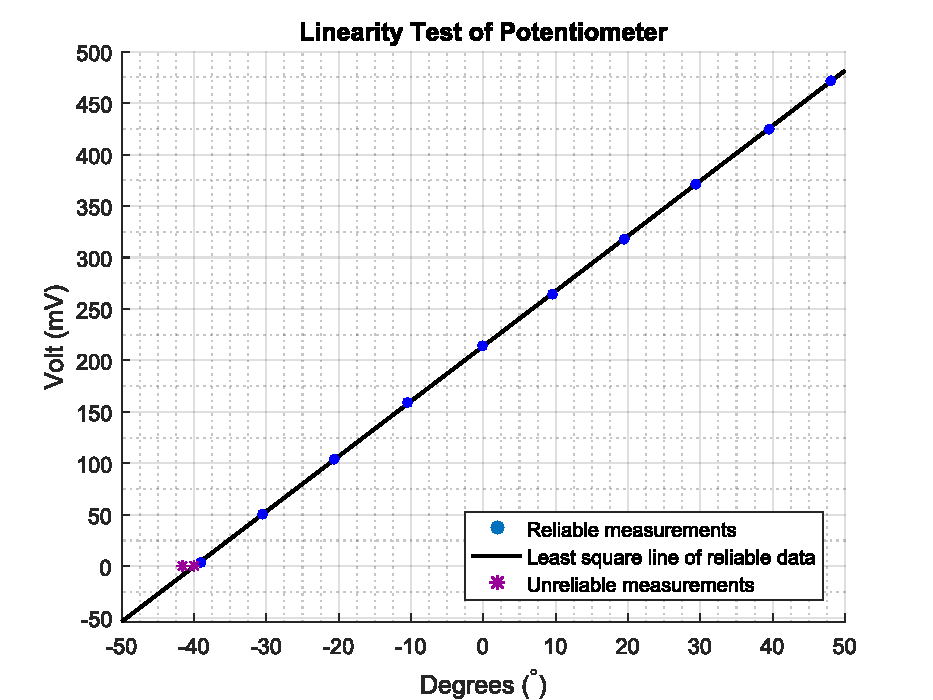
\includegraphics[scale=0.5]{figures/linearityOfPotmeterTest2-1}
	\caption{Result of the linearity test}
	\label{linearityOfPotmeterTest}
\end{figure}


\textbf{- Range Test}
An additional test is done to find the conversion from voltage to angle of the potentiometer. It is also tested if there is an offset that has to be taken into account. The detailed description of this test is found in \appref{app:potentiometerRes}
%It is also needed a test to find the conversion from voltage to angle along with potential offset (see ).

\begin{minipage}{\linewidth}
  	\begin{minipage}{0.45\linewidth}
  		\begin{figure}[H]
  			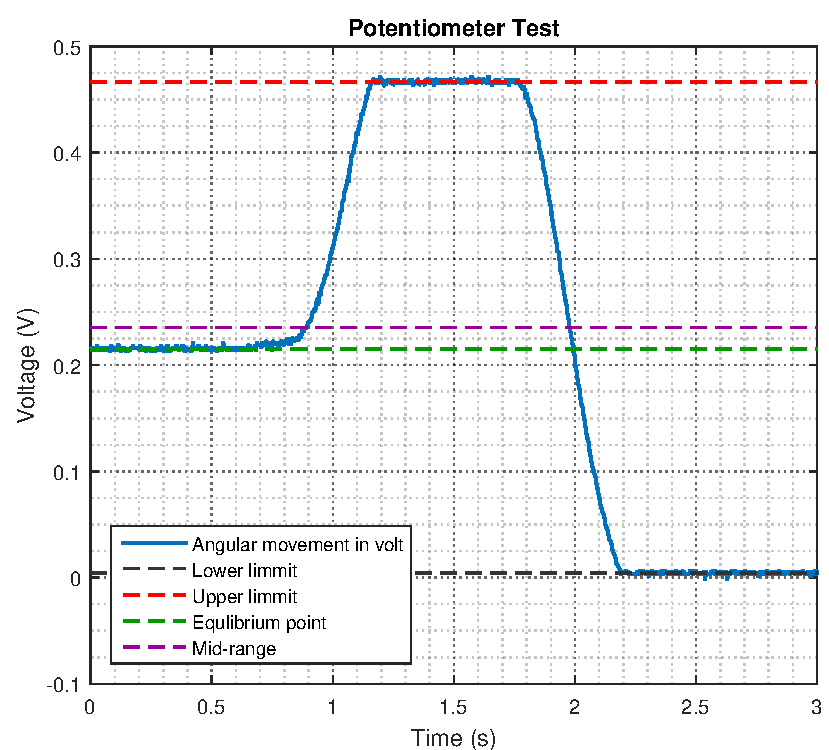
\includegraphics[scale=.5]{figures/PotentiometerResolution}
  			\centering
  			\captionsetup{justification=centering}
  			\captionof{figure}{\\Potentiometer measurements in volts}
  			\label{PotentiometerResolution}
  		\end{figure}\vspace{-5mm}
  	\end{minipage}
  	\hspace{0.03\linewidth}
  	\begin{minipage}{0.45\linewidth}
  		\begin{figure}[H]
  		%\vspace{.5cm}
  			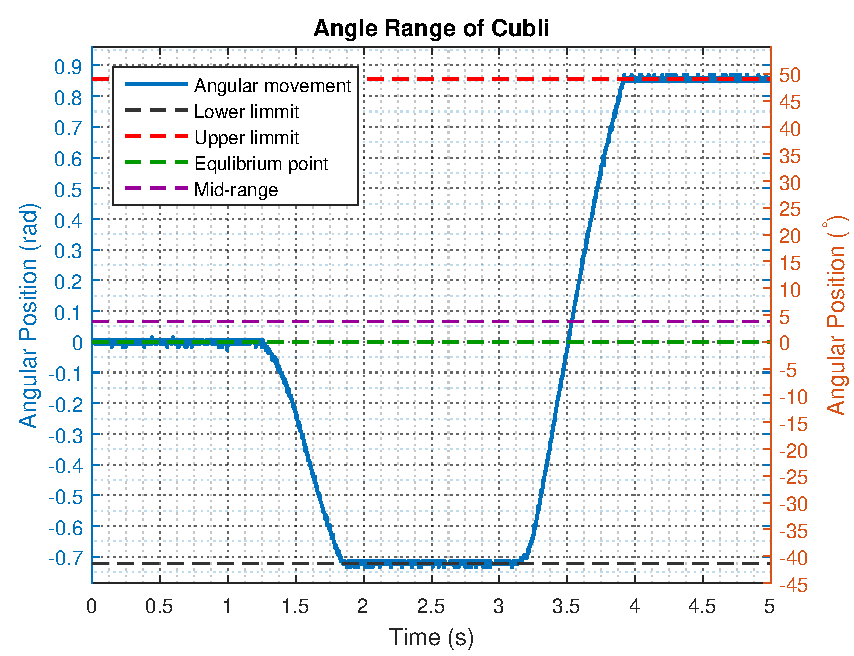
\includegraphics[scale=.5]{figures/PotentiometerResolutionDegRad}
  			\centering
  			\captionsetup{justification=centering}
  			\vspace{-.5cm}
  			\captionof{figure}{\\Potentiometer measurements converted to radians and degrees}
  			\label{PotentiometerResolutionRadDeg}
  		\end{figure}\vspace{-5mm}
  	\end{minipage}
\end{minipage}

The results of this test is shown above in \figref{PotentiometerResolution}, where the reference lines reveals an offset between the middle of the range and the equilibrium point of the Cubli frame.\\
This offset, also seen angle offset on \figref{PotentiometerResolutionRadDeg}, exists in the physical position of the frame. When the frame is standing in its equilibrium position it is displaced by approximately \SI{0,068}{rad} due to uneven distribution of mass around its center.\\
This results in a \SI{0,853}{rad} range to one side of the optimal position and \SI{0,717}{rad} on the other.\\
It is chosen that the angle-offset must be accounted for such that the equilibrium position of the frame is at angle 0.

%Equilibrium point has been tested to have a range of 1 degree and the angle between the base and the frame is 42,5 degree. To avoid complications it is chosen that the angle-offset must be accounted for such that the equilibrium position of the frame is at 0 degree angle. This results in a 48,9 degree range to one side of the optimal position and 41,1 degree on the other.

\subsection{Inertial Measurement Unit}
The Motion Processing Unit (MPU) contains a triple axis accelerometer and gyro integrated in the same chip mounted on the breakout board from SparkFun.

The gyro has a sensitivity up to 131 LSBs/dps and a full-scale range of ±250, ±500, ±1000, and ±2000dps, while the accelerometer has a programmable full scale range of ±2g, ±4g, ±8g and ±16g.

The input voltage can be between 2,3 and 3,4V, and it includes embedded algorithms for run-time bias and compass calibration.

The unit collects gyroscope and accelerometer data while synchronizing data sampling at a user defined rate, and it uses Inter Integrated Circuit (\si{I^2C}) protocol for communication, whose speed can be up to 400 kHz. 


%The Motion Processing Unit (MPU) is a triple axis accelerometer and gyro mounted integrated in the same chip mounted on the breakout board from SparkFun. %This is also called 6 Degrees of Freedom (6-DOF).
%
%The MPU 6050 is a sensor based on Micro Electro Mechanical Systems (MEMS) technology. This chip uses Inter Integrated Circuit (\si{I^2C}) protocol for communication, and is using \si{I^2C} speed up to 400 kHz. 
%
%The unit has a built-in temperature sensor which is used internally for more accurate measurements.
%embedded algorithms for run-time bias and compass calibration so no user calibration are required.
%The unit collects gyroscope and accelerometer data while synchronizing data sampling at a user defined rate. 

%For more precision measurement of the gyroscope and accelerometer, the unit can be programmed for the measurement of different intervals for the gyroscope from ±250 to ±2000 Degrees Per Second (DPS) and for a accelerometer range of ±2 g to ±16 g.
%\fxnote{This should be in the appendix: The measurements of the gyroscope can be set from \si{\pm250} to \si{\pm2000} \si{deg \cdot s^{-1}}, the chosen configuration is found in... and what is in the appendix should be here\appref{app:}.}

%The unit have built in 16-bit ADC converters for digitizing the gyroscope and accelerometer outputs and a digitally low-pass filter that can be programmed.

% MPU-6050 have a buffer of 1024 Byte. The buffer is First In First Out (FIFO) type and is reducing timing requirements on the system processor.

%The Digital Motion Processor (DMP) is capable of processing, so the digital output of the unit can be calculated as 6-Axis or 9-Axis MotionFusion on the unit. The output-data can come as rotation matrix, quaternion, Euler Angle, or raw data format. 

%The MPU’s calculated output to the system processor can also include heating data from a digital 3-axis third party magnetometer.

%\subsection{Planning of different test.}
%The Cubli is analyzed so the parameters is confirmed and also to find the changes that have been made after the electronic board has been added to the frame during the last parameters measurement. For this reason, different tests will be made on the Cubli to find the different parameters and sensor inputs that will be used in making a model of the system.